
\section{Building the unit cell}
\label{buildingunitcell}

Once we have selected $models$ for \ttt{metHgb} $\alpha$ and $\beta$ subunits, we can regenerate the smallest asymmetrical element (unit cell) of the starting volume. With this aim $Chimera$ \ttt{rigid fit} and assessment - refinement -assessment protocols will be used.\\ 

\begin{itemize}
 \item Protocol \scommand{chimera rigid fit} to generate the unit cell of human \ttt{metHgb}:\\
 
    Open again $Chimera$ \ttt{rigid fit} protocol and following already indicated instructions, include this time $models$ for \ttt{metHgb} $\alpha$ and $\beta$ subunits (\ffigure{fig:chimera_rigid_fit} (3 and 4)). Firstly, perform the rigid fit of the extracted unit cell (output\_volume.mrc) and both subunits \#2 and \#3, by using \ttt{Tools -> Volume Data -> Fit in Map} in $Chimera$ (\ffigure{fig:chimera_rigid_fit_A_B}). Next, create a single atomic structure by selecting models \#2 and \#3 in $Chimera$ \ttt{Model Panel} and pressing \ttt{Copy/Combine} command in the right column. A new model \#4 is shown in $Chimera$ \ttt{Model Panel}. Finally, save this fitted structure writing in $Chimera$ command line:\\
    \ttt{scipionwrite model \#4 refmodel \#1 saverefmodel 0}\\
    
    \begin{figure}[H]
    \centering 
    \captionsetup{width=.7\linewidth} 
    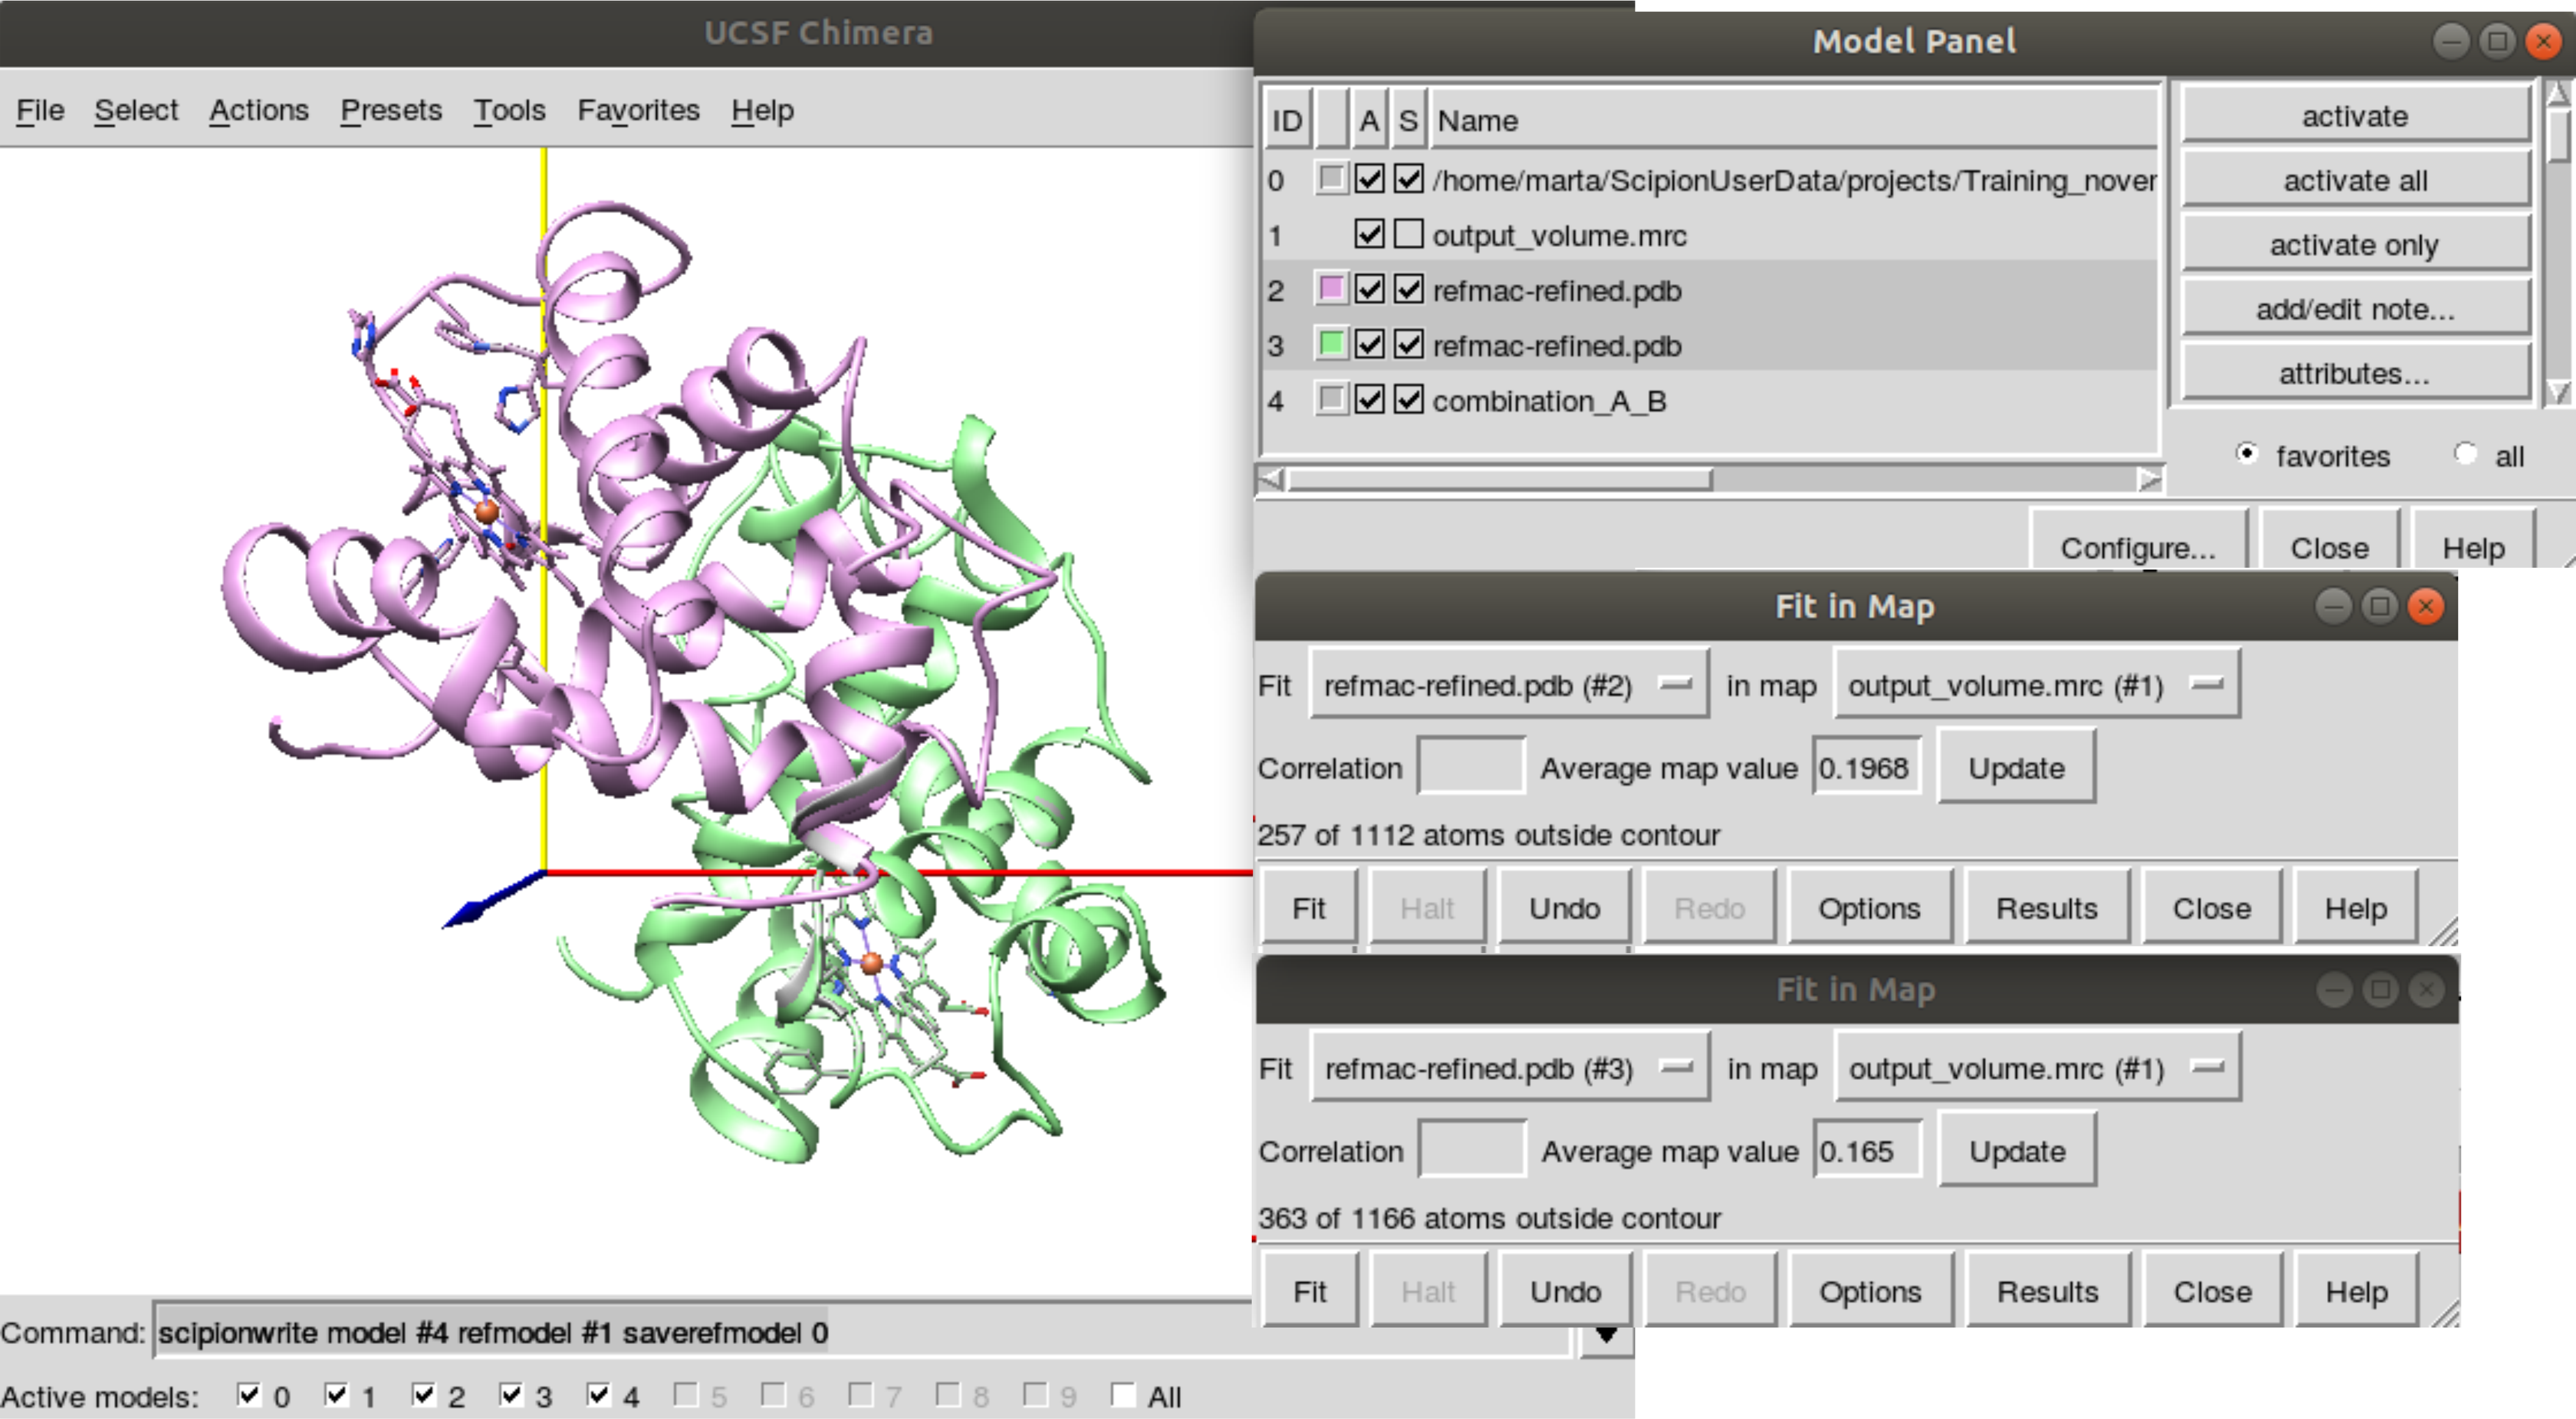
\includegraphics[width=0.90\textwidth]{Images/Fig40}
    \caption{Generation of the human \ttt{metHgb} unit cell $model$.}
    \label{fig:chimera_rigid_fit_A_B}
   \end{figure}
    
 \item Validation protocols to select the best $model$ of the human \ttt{metHgb} unit cell:\\
 
 $EMRinger$ and $MolProbity$ validation statistics should be computed for the new $model$ of human \ttt{metHgb} unit cell, generated by combining \ttt{metHgb} $\alpha$ and $\beta$ subunits. Appendix \ref{app:solutions} (\textbf{Question \ref{buildingunitcell}\_1}) contains a statistics table for the unit cell $model$ (\ttable{table:refmac_question_11}). We can try to improve those statistics by additional refinement processes. By performing refinement in real space with $Phenix$ and, additionally, in reciprocal space with $Refmac$, some of the statistics will result improved. \ttable{table:refmac_question_11} contains also RMSD values computed in a similar way as we have seen for $\alpha$ and $\beta$ subunits, considering as fixed structure chains A and B from \ttt{5NI1} atomic structure. In this tutorial, we have selected the unit cell $model$ generated by $Phenix$ \ttt{real space refine} (modified parameters) because it shows most of best statistics (\ccmask, $EMRinger$ \ttt{score} and $MolProbity$ values). Exceptionally, RMSD regarding the published structure yields the worst value.
 
\end{itemize}

